
\section{Center of Mass}
\subsection{Center of Mass Defined by Moment Integrals}\label{CoM}

Let $R$ be a region bounded above by $f(x)$, below by $g(x)$, on the left by $x=a$, and on the right by $x=b$.  Let $(\bar{x},\bar{y})$ be the center of mass of $R$, a region of area $m$.  The formulas for the $x$- and $y$- coordinates of the \moment{center of mass} of a 2D plate in the shape of $R$ are as follows:

\begin{align*}
 \bar{x}&= \frac{1}{m} \int_{x=a}^{x=b} x\left(f(x)-g(x)\right) \dif x\\
 \bar{y}&= \frac{1}{m} \int_{x=a}^{x=b} \frac{1}{2}\left(f(x)+g(x)\right)\left(f(x)-g(x)\right)\dif x
\end{align*} 

\vspace{.1in}

The \moment{integrals} above are often referred to as \emph{\integ{moments}}, a term physicists use to describe the turning effect of a force.  Thus, the definition is often stated in terms of these moment integrals $M_y$ and $M_x$. We define the following abbreviations:

\begin{align*}
 m&=  \int_{x=a}^{x=b} \left(f(x)-g(x)\right) \dif x\\
 M_y&=  \int_{x=a}^{x=b} x\left(f(x)-g(x)\right) \dif x\\
 M_x&=  \int_{x=a}^{x=b} \frac{1}{2}\left(f(x)+g(x)\right)\left(f(x)-g(x)\right)\dif x
\end{align*} 
This gives a short formula for the center of mass of the region $R$.

\FormulaBox{Center of Mass}{The center of mass of $R$ is the point $\left(\bar{x},\bar{y}\right)=\left(M_y/m,M_x/m\right)$.}
The \centerofmass{physical interpretation} of the center of mass is quite nice; it is the point where we could theoretically balance our 2D plate on a narrow post.  Also, in many physics or engineering applications, one can replace the entire figure with a point mass located at the center of mass.  This simplifies many otherwise difficult problems.  If you are ever going to take the \emph{Fundamentals of Engineering} exam, this is a huge trick people use!

Here we make the simplifying assumption that the \area{unit of mass} we are using is 1 unit of mass per unit of area.  Thus, $m$ can be computed as the area of $R$.

	\begin{center}
		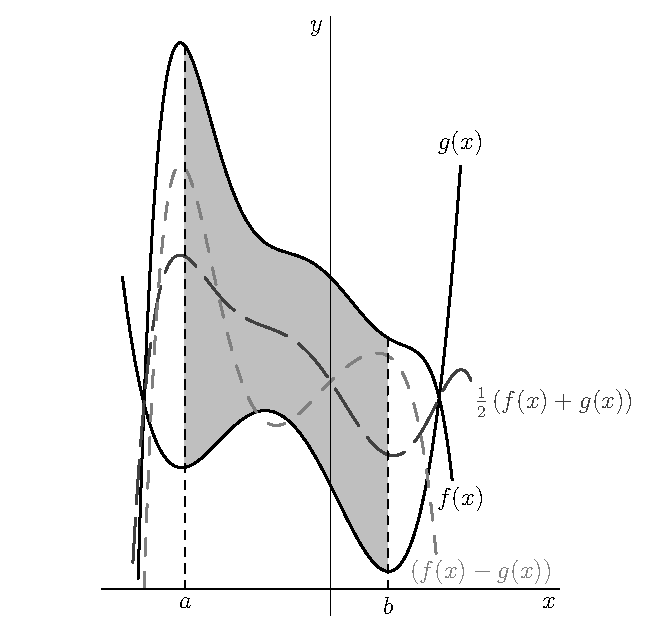
\includegraphics[width=300pt]{ChapterGeom/Figures/centmass.eps}
	\end{center}

These formulas are plausible, as in some sense we are measuring the tendency to rotate about an axis.  We can see the first integral is accumulating $x$ (the length of the torque arm) times $(f(x)-g(x))$, which is measuring the height of the figure at location $x$.  The second integral is much less intuitive, though we can see it again as accumulating the heights times the average of the $y$ coordinate of the boundaries, which in aggregate gives us a measure of the central tendency of the vertical component of the figure.  These formulas will be proven in Calc III via double-integration.

\begin{example}{Center of Mass of a Cosine Gumdrop}\label{gumdrop}
Consider the region $R$ bounded by the graphs of $y=0$ and $y=\cos(x)$ between $x=-\pi/2$ and $x=\pi/2$.

To find the center of mass, we have three quantities we need to compute: the area $m$, the $y$-axis moment $M_y$, and the $x$-axis moment $M_x$.  We compute each now, using $f(x)=\cos(x)$ and $g(x)=0$:

\begin{itemize}
\item $m=\int_{x=-\pi/2}^{ x=\pi/2}\left(\cos(x)-0\right)\dif x = \left.\sin(x) \right]_{x=-\pi/2}^{x=\pi/2}=\sin\left(\frac{\pi}{2}\right)-\sin\left(-\frac{\pi}{2}\right)=1-(-1)=2$
\item $M_y=\int_{x=-\pi/2}^{x=\pi/2}x\left(\cos(x)-0\right)\dif x =\left.x\sin(x)+\cos(x)\right]_{x=-\pi/2}^{x=\pi/2} = \frac{\pi}{2}-\left(-\frac{\pi}{2}(-1)\right)=0 $
\item $M_x=\int_{x=-\pi/2}^{x=\pi/2}\frac{\left(\cos(x)+0\right)}{2}\left(\cos(x)-0\right)\dif x =\left.\frac{1}{2}\left(\frac{x}{2}-\frac{1}{4}\sin\left(2x\right)\right)\right]_{x=-\pi/2}^{x=\pi/2}=\frac{\pi}{4} $ 
\end{itemize}
Thus, the center of mass of $R$ is $$\left(\bar{x},\bar{y}\right)=\left(M_y/m,M_x/m\right)=\left(0/2,\left(\pi/4\right)/2\right)=\left(0,\pi/8\right). $$ 
\begin{center}
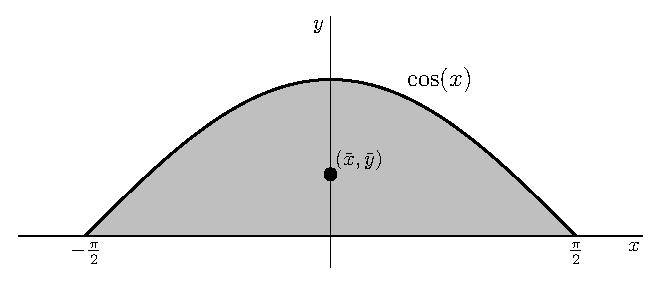
\includegraphics[width=300px]{ChapterGeom/Figures/CosineGumdrop}
\end{center}
\end{example}

We now gather a little geometric intuition on the above example (do we \ldots reflect?) as well as check the details of the integration.

\begin{exercise}{Integration and Intuition \Coffeecup}
In the above example\ldots
\begin{itemize}
\item \ldots how could we have predicted that $\bar{x}$ would be zero just from the shape of the region?

\solushun{The region is symmetrical about the $y$-axis, so its center of mass would be right on the $y$-axis, at $x=0$.\\}{.5in}

\item \ldots how could we have predicted that $\bar{y}$ should be a bit less than one half?  Specifically, think about how tall the region $R$ is and then ask if the region is more top heavy or more bottom heavy?  Verify that $\pi/8$ is in fact a bit less than one half.

\solushun{The region is 1 unit tall because that is the max value of $\cos(x)$. It is more bottom-heavy since it narrows to the top. Roughly, $\frac{\pi}{8}$ is less than $\frac{1}{2}$ because $\frac{3}{6}=\frac{1}{2}$, and $\pi$ is only slightly greater than 3, while 8 is a fair bit more than 6. A more precise calculation gives $\frac{\pi}{8}=0.39$\\}{.5in}

\item \ldots the $M_y$ integral required use of Integration by Parts.  Show the details of this antidifferentiation.

\solushun{
\begin{align*}
M_y=\int_{x=-\pi/2}^{x=\pi/2}x\left(\cos(x)-0\right)\dif &= \int_{x=-\pi/2}^{x=\pi/2} x\cos(x) \dif x\\
\text{Let }u=x,\dif u=\dif x, v=\sin(x), \dif v=\cos(x)\\
&=x\sin(x)-\int_{x=-\pi/2}^{x=\pi/2} \sin(x)\dif x\\
&=\left.x\sin(x)+\cos(x)\right]_{x=-\pi/2}^{x=\pi/2} = \frac{\pi}{2}-\left(-\frac{\pi}{2}(-1)\right)=0 \end{align*}
}{.5in}

\item \ldots the $M_x$ integral required use of a trig identity.  Which identity was used?  Show the details of this antidifferentiation.

\solushun{We used the identity $\cos^2\theta=\frac{1}{2}\left(1+\cos2\theta\right)$.

\begin{align*}
M_x=\int_{x=-\pi/2}^{x=\pi/2}\frac{\left(\cos(x)+0\right)}{2}\left(\cos(x)-0\right)\dif x &=\int_{x=-\pi/2}^{x=\pi/2}\frac{1}{2}\cos^2(x)\dif x\\
&=\int_{x=-\pi/2}^{x=\pi/2}\frac{1}{2}\left(\frac{1}{2}\right)(1+\cos(2x))\dif x\\
&=\left(\frac{1}{2}\right)\left(\frac{1}{2}\right)\left.(x+\frac{1}{2}\sin(2x))\right|_{x=-\pi/2}^{x=\pi/2} \\
&=\left.\frac{1}{2}\left(\frac{x}{2}-\frac{1}{4}\sin\left(2x\right)\right)\right|_{x=-\pi/2}^{x=\pi/2}\\
&=\frac{\pi}{4}
\end{align*}
}{.5in}

\end{itemize}
\end{exercise}
\begin{exercise}{A Sine Gumdrop \Coffeecup \Coffeecup}
Consider the region $R$ bounded by the graphs of $y=0$ and $y=\sin(x)$ between $x=0$ and $x=\pi$.  \begin{itemize}
\item Based on the center of mass computed in Example \ref{CoM}.\ref{gumdrop}, what would you suspect this new center of mass to be?  

\solushun{
Since the graph of $\sin(x)$ has the same shape as the graph of $\cos(x)$, only shifted to the right $\frac{\pi}{2}$ units along the $x$-axis, we know that the center of mass will be the same as that of the region above, except shifted to the right $\frac{\pi}{2}$. So the center of mass will be $(\frac{\pi}{2},\frac{\pi}{8})$.\\
}{1in}

\item  Verify or refute your suspicion by computing the center of mass using moment integrals. 

\solushun{
$m=\int_{x=0}^{ x=\pi}\left(\sin(x)-0\right)\dif x = \left.-\cos(x) \right]_{x=0}^{x=\pi}=-\cos(\pi)-(-\cos(0)=-(-1)-(-1)=2$
\begin{align*}
M_y=\int_{x=0}^{x=\pi}x\left(\sin(x)-0\right)\dif &= \int_{x=0}^{x=\pi}x\sin(x) \dif x\\
&\text{Let }u=x,\dif u=\dif x, v=-\cos(x), \dif v=\sin(x)\\
&=-x\cos(x)+\int_{x=0}^{x=\pi} \cos(x)\dif x\\
&=\left.-x\cos(x)+\sin(x)\right]_{x=0}^{x=\pi}\\
&=(-\pi(-1)+0)-(0+0)= \pi
\end{align*}
\begin{align*}
M_x=\int_{x=0}^{x=\pi}\frac{\left(\sin(x)+0\right)}{2}\left(\sin(x)-0\right)\dif x &=\int_{x=0}^{x=\pi}\frac{1}{2}\sin^2(x)\dif x\\
&=\int_{x=0}^{x=\pi}\frac{1}{2}\left(\frac{1}{2}\right)(1-\cos(2x))\dif x\\
&=\left(\frac{1}{2}\right)\left(\frac{1}{2}\right)\left.(x-\frac{1}{2}\sin(2x))\right]_{x=0}^{x=\pi} \\
&=\left.\frac{1}{2}\left(\frac{x}{2}-\frac{1}{4}\sin\left(2x\right)\right)\right]_{x=0}^{x=\pi}\\
&=\frac{1}{2}\left(\frac{\pi}{2}-\frac{1}{4}\sin\left(2\pi\right)-\left(\frac{0}{2}-\frac{1}{4}\sin\left(0\right)\right)\right)\\
&=\frac{\pi}{4}
\end{align*}
Center of mass$=(\bar{x},\bar{y})=(M_y/m,M_x/m)=(\frac{\pi}{2},\frac{\pi}{8})$.

}{2in}
\AnswerKeyEntry{The sine gumdrop is just a translation $\pi/2$ units to the right of the cosine gumdrop.  So, we would expect the center of mass to have the same $y$-coordinate but have an $x$-coordinate that is $\pi/2$ units larger.  Indeed, when computed with the moment integrals, we get $\left(\bar{x},\bar{y}\right)=\left(\pi/2,\pi/8\right)$. }
\end{itemize}

\end{exercise}

We now play with center of mass for a few of our common shapes.

\subsection{The Rectangle}

Suppose we have a \centerofmass{rectangle} of width $w$ and height $h$.  If we coordinatize the rectangle by placing the lower-left corner at the origin and the bottom side on the positive $x$-axis, we would expect that the center of mass should come out to be the point $(w/2,h/2)$ since that intuitively is the ``middle" of our rectangle.  Let's try out the integrals and verify this is indeed what we get.  Specifically:

	\begin{center}
		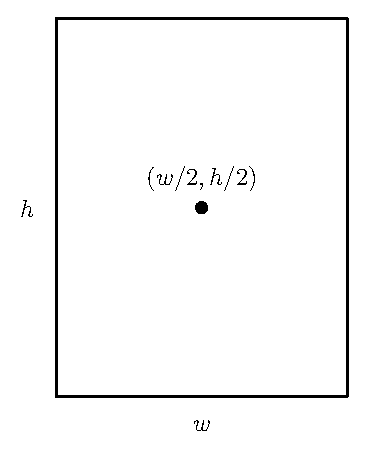
\includegraphics[width=150pt]{ChapterGeom/Figures/rectangle.eps}
	\end{center}
\begin{exercise}{A Rectangle \Coffeecup \Coffeecup}

\begin{itemize}

\item Let $f(x)=h$ the constant function whose graph is a horizontal line at height $h$, be the top of the rectangle.  Let $g(x)=0$, the constant function whose graph is a horizontal line at height zero, be the bottom of the rectangle.  Let the lines $x=0$ and $x=w$ be the left and right boundaries of the rectangle.  Sketch this figure below.

    \solushun{
        \begin{center}
            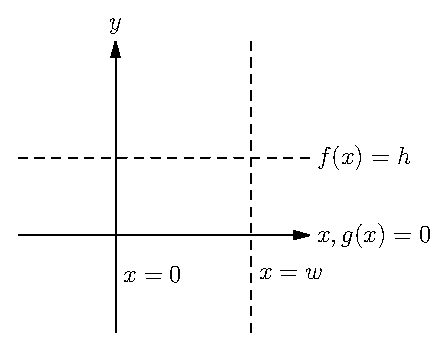
\includegraphics[width=150pt]{ChapterGeom/Figures/rectangle-soln.eps}
        \end{center}
    }{2in}

\item Use our center of mass formulas to compute $(\bar{x},\bar{y})$ and verify that it is in fact $(w/2,h/2)$.

\solushun{\\
$M_y=\int_{x=0}^{x=w}x(f(x)-g(x))\dif x=\int_{x=0}^{x=w}hx\dif x=\left.\frac{1}{2}hx^2\right|_{x=0}^{x=w}=\frac{1}{2}hw^2$\\

$M_x=\int_{x=0}^{x=w}\frac{\left(h\right)}{2}\left(h\right)\dif x=\left.\frac{1}{2}h^2x\right|_{x=0}^{x=w}=\frac{1}{2}h^2w$ \\

$m=\int_{x=0}^{x=w}h\dif x =\left.hx\right|_{x=0}^{x=w}=hw$\\
\\
$\bar{x}=M_y/m=\frac{hw^2}{2hw}=\frac{w}{2}$\\
$\bar{y}=M_x/m=\frac{h^2w}{2hw}=\frac{h}{2}$\\
\\
$COM=(\frac{w}{2},\frac{h}{2})$\\
}{3in}

\end{itemize}
\end{exercise}

\subsection{The Parallelogram}

	\begin{center}
		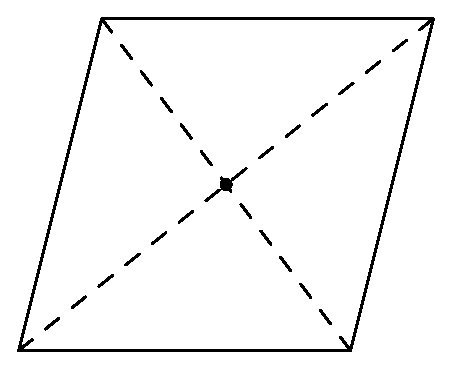
\includegraphics[width=150pt]{ChapterGeom/Figures/parallel.eps}
	\end{center}

Again by intuition, we would imagine the center of mass of a \centerofmass{parallelogram} should be at the intersection of the diagonals.  Let's see if this is in fact where the center of mass of a parallelogram must lie.  We will do this in three steps:
\begin{exercise}{Parallelogram \Coffeecup \Coffeecup}

\begin{itemize}

\item Coordinatize the parallelogram.  Choosing ``nice'' coordinates for our figure is the first step.  Without loss of generality, we can make one corner of our parallelogram to be the origin and choose one side to lie on the positive $y$-axis, much like the rectangle.  The beauty of this is then the parallelogram is fully determined by only three arbitrary parameters, the horizontal and vertical coordinates of the upper right corner, and the vertical coordinate of the upper left corner.  Call these $a$, $b$, and $c$ respectively.

    \solushun{
        \begin{center}
            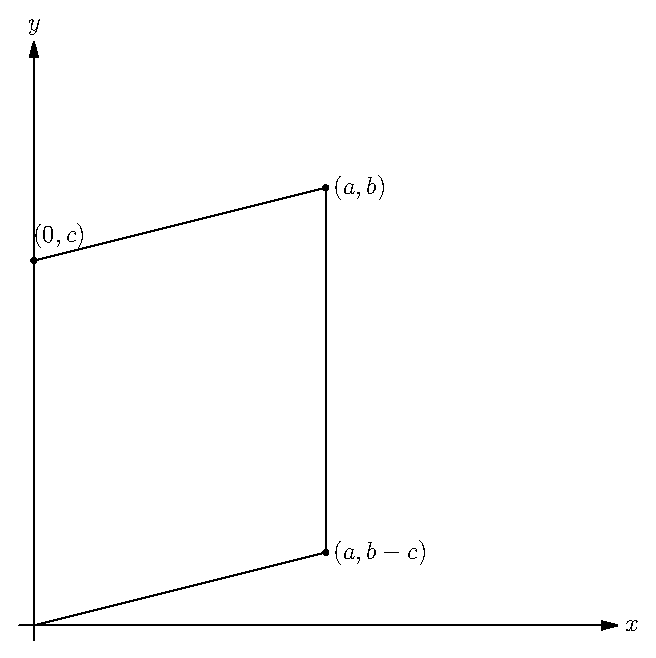
\includegraphics[width=200pt]{ChapterGeom/Figures/parallel-soln.eps}
        \end{center}
    
    }{2in}
 
\item Compute linear equations for the diagonals in terms of $a,b,$ and $c$.  Solve a simultaneous system of linear equations to find the coordinates of the intersection of these lines.

\solushun{
$$l_1:y=\frac{b-0}{a-0}x+0=\frac{b}{a}x$$
$$l_2:y=\frac{(b-c)-c}{a-0}x+c=\frac{b-2c}{a}x+c$$
Setting $l_1=l_2$ we may solve for $x$.

$$\frac{b}{a}x=\frac{b-2c}{a}x+c$$
$$\frac{b-b+2c}{a}x=c$$
$$\frac{2c}{a}x=c$$
$$x=\frac{a}{2}$$

Plugging this back into $l_2$, we get $y=\frac{b}{2}$. So using intersecting diagonals, we get the center of mass at $(\frac{a}{2},\frac{b}{2})$.\\}{2in}

\item Use the integrals for center of mass to compute the actual center of mass.  See if it agrees with the coordinates of the point of intersection computed above.

\solushun{
$$M_y=\int_{x=0}^{x=a}x\left(\frac{b-c}{a}x+c-\frac{b-c}{a}x\right)\dif x=\int_{x=0}^{x=a} xc=\left.\frac{1}{2}cx^2\right|_{x=0}^{x=a}=\frac{1}{2}ca^2$$

\begin{align*}
M_x&=\int_{x=0}^{x=a}\frac{1}{2}\left(\frac{b-c}{a}x+c+\frac{b-c}{a}x\right)\left(\frac{b-c}{a}x+c-\frac{b-c}{a}x\right)\dif x\\
&=\int_{x=0}^{x=a}\frac{1}{2}\left(\frac{2(b-c)}{a}x+c\right)c\dif x\\
&=\int\frac{bc-c^2}{a}x+\frac{1}{2}c^2\dif x\\
&=\left.\frac{bc-c^2}{2a}x^2+\frac{1}{2}xc^2\right]_{x=0}^{x=a}\\
&=\frac{abc-ac^2}{2}+\frac{1}{2}ac^2=\frac{abc}{2}
\end{align*}

\begin{align*}
m=\int_{x=0}^{x=a}\frac{b-c}{a}x+c-\frac{b-c}{a}x\dif x=\int_{x=0}^{x=a} c=\left.cx\right|_{x=0}^{x=a}=ca
\end{align*}

$$\bar{x}=M_y/m = \frac{ca^2}{2ca}=\frac{a}{2}$$
$$\bar{y}=M_x/m = \frac{abc}{2ac}=\frac{b}{2}$$}{3in}
\AnswerKeyEntry{The diagonals have the equations $$ y=\frac{b}{a}x \text{ and } y=\frac{b-2c}{a}x+c$$ with intersection point $(a/2,b/2)$, which is also the center of mass of the region.}
\end{itemize}

\end{exercise}
Ok nice, so it did work out to be the same!  Well it kind of had to there, right?  I mean what else could the center of mass of a parallelogram have been?

\subsection{The Triangle}

And now for a case where the end of the story is far less predictable!  Consider the triangle.  For the \centerofmass{triangle} there are \emph{four} completely reasonable geometric guesses as to what the ``center" of a triangle could be.  

\begin{exercise}{Different Notions of Center of a Triangle \Coffeecup}

Sketch corresponding diagrams for four beautiful theorems of Euclidean geometry.

\begin{itemize}

\item The altitudes of a triangle intersect in a point.  (This point is called the \emph{orthocenter}.)

    \solushun{
        \begin{center}
            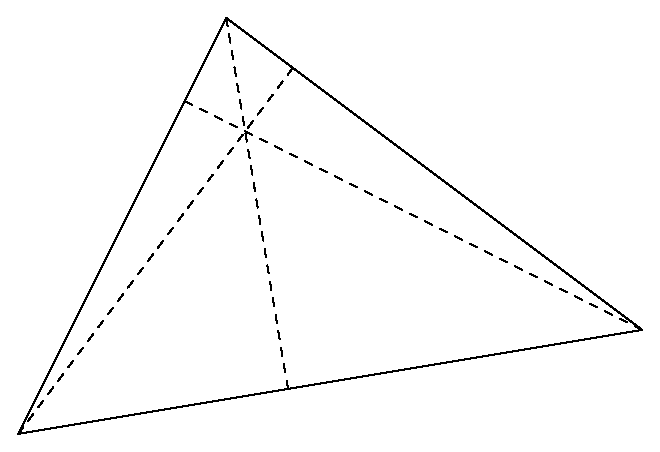
\includegraphics[width=200pt]{ChapterGeom/Figures/orthotri.eps}
        \end{center}
    
    }{2in}

\item The medians of a triangle intersect in a point.  (This point is called the \emph{barycenter}.)

    \solushun{
        \begin{center}
            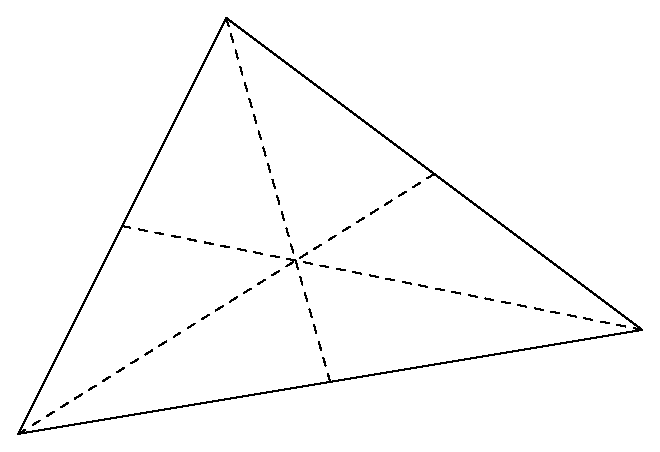
\includegraphics[width=200pt]{ChapterGeom/Figures/barytri.eps}
        \end{center}
    
    }{2in}

\item The perpendicular bisectors of a triangle intersect in a point.  (This point is called the \emph{circumcenter}.)

    \solushun{
        \begin{center}
            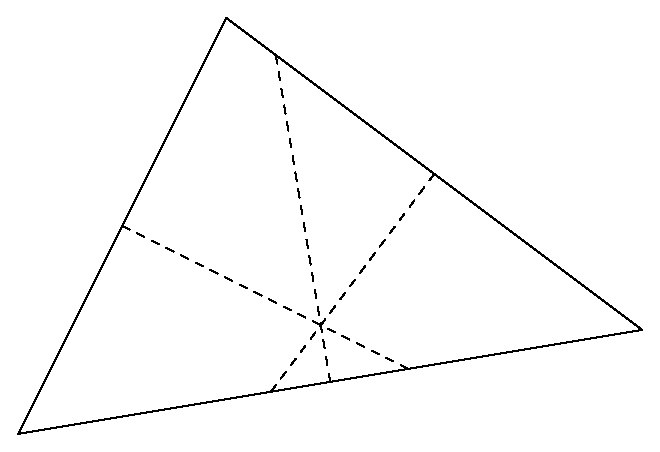
\includegraphics[width=200pt]{ChapterGeom/Figures/circumtri.eps}
        \end{center}
    
    }{2in}

\item The angle bisectors of a triangle intersect in a point.  (This point is called the \emph{incenter}.)

    \solushun{
        \begin{center}
            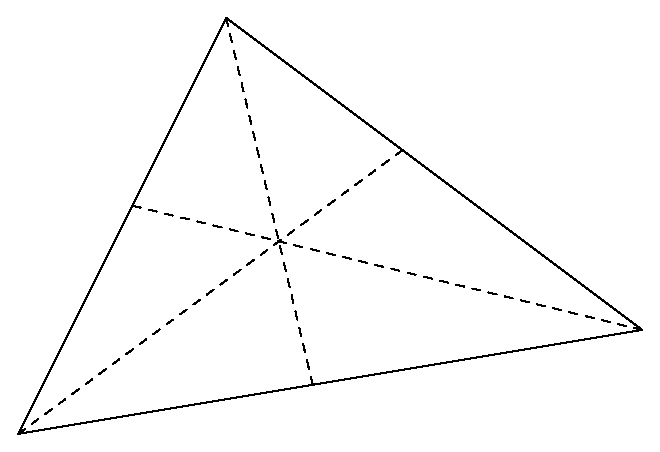
\includegraphics[width=200pt]{ChapterGeom/Figures/intri.eps}
        \end{center}
    
    }{2in}

\end{itemize}
\end{exercise}

Of these different notions of ``center'' of a triangle, which one is actually the center of mass?  Or is it something different entirely that is not on our list of guesses above?  Well, let's figure it out.  The steps for determining this are essentially the same as for the parallelogram.
\begin{exercise}{The Triangle \Coffeecup \Coffeecup \Coffeecup}

\begin{itemize}

\item Coordinatize the triangle.  Choosing ``nice'' coordinates for our figure is the first step.  Without loss of generality, we can make one corner of our triangle to be the origin and choose one side to lie on the positive $y$-axis, much like the rectangle and parallelogram.  Now the triangle is fully determined by only three arbitrary parameters, the horizontal and vertical coordinates of the only corner not on the $y$-axis, and the $y$-coordinate of the point on the $y$-axis but not at the origin.  Similar to the parallelogram, respectively call these $a$,$b$, and $c$.  Note how helpful this is; a generic triangle in the plane would be determined by six parameters! (two per corner)

\solushun{\hfill
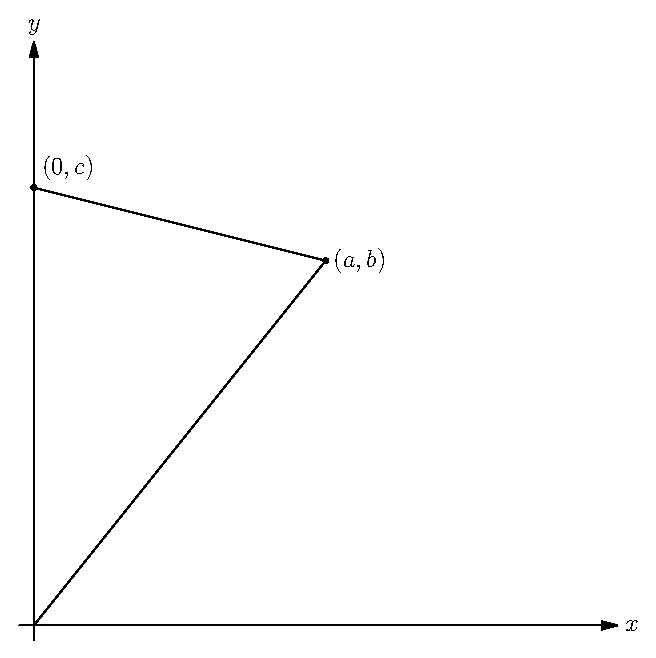
\includegraphics[width=300px]{ChapterGeom/Figures/trianglecoords_cropped.eps}
}{2in}

\item Note that for extreme cases, the circumcenter and orthocenter can actually lie outside of the triangle.  This means these are likely to be incorrect guesses, as we would intuitively think the center of mass of the triangle should always lie inside the triangle itself.  Thus, we won't expend effort trying to find coordinates for the orthocenter or circumcenter.  To confirm this, draw one example of a triangle below that has orthocenter outside and one example of a triangle that has circumcenter outside.

\vspace*{2in}

\item Going down the list, let's find the barycenter.  The process is the same as above.  We find equations for two of the medians and find their point of intersection.  (Note that thanks to Euclid's theorem that the three medians intersect in a point, it is not necessary to use the equation for the third median as it is guaranteed to pass through the same point of intersection.)

\solushun{First, find the median from $(0,c)$ to $\left(\frac{a}{2},\frac{b}{2}\right)$. The y-intercept of this line will be $c$ and the slope is
$$\frac{c-\frac{b}{2}}{0-\frac{a}{2}}=\frac{b-2c}{a}.$$
Then the slope-intercept equation for the first median is
$$y=\frac{b-2c}{a}x+c.$$

Next, find either of the other two medians. We'll choose the one from $\left(0,\frac{c}{2}\right)$ to $(a,b)$, since it seems easier to compute. The $y$-intercept is $\frac{c}{2}$. The slope is
$$\frac{\frac{c}{2}-b}{0-a}=\frac{2b-c}{2a}.$$
The the slope intercept equation for the line is
$$y=\frac{2b-c}{2a}x+\frac{c}{2}.$$

Last, we can find the point of intersection by setting the two equations equal.
\begin{align*}
\frac{b-2c}{a}x+c&=\frac{2b-c}{2a}x+\frac{c}{2}\\
(2a)\left(\frac{b-2c}{a}x+c\right)&=\left(\frac{2b-c}{2a}x+\frac{c}{2}\right)(2a)\\
(2b-4c)x+2ac&=(2b-c)x+ac\\
2bx-4cx+2ac&=2bx-cx+ac\\
-3xc+ac&=0\\
x&=\frac{-ac}{-3c}=\frac{a}{3}
\end{align*}

Plug this $x$ value into either equation to find $y$.
$$y=\frac{b-2c}{a}\left(\frac{a}{3}\right)+c=\frac{b+c}{3}$$

So the barycenter is located at $\left(\frac{a}{3},\frac{b+c}{3}\right)$.\\ }{4in}

\item Use the integrals for center of mass to compute the actual center of mass. See if it agrees with the coordinates of the point of intersection computed above.

\solushun{
First, get the mass:
\begin{align*}
m=\int_0^a \frac{b-c}{a}x +c -\frac{b}{a}x \dif x&=\int_0^a\frac{-c}{a}x+c \dif x\\
&=\left[\frac{-c}{2a}x^2+cx\right]_0^a\\
&=\frac{-ac}{2}+ac\\
&=\frac{ac}{2}
\end{align*}

Next, let's calculate each moment.

\begin{align*}
M_y=\int_0^a x[f(x)-g(x)]\dif x&=\int_0^a\frac{-c}{a}x^2+cx \dif x\\
&=\left[\frac{-c}{3a}x^3+\frac{c}{2}x^2\right]_0^a\\
&=\frac{-a^2c}{3}+\frac{a^2c}{2}\\
&=\frac{-2a^2c+3a^2c}{6}\\
&=\frac{a^2c}{6}
\end{align*}

\begin{align*}
M_x=\int_0^a\frac{1}{2}[f(x)-g(x)][f(x)+g(x)]\dif x&=\frac{1}{2}\int_0^a\left(\frac{-c}{a}x+c\right)\left(\frac{b-c}{a}x+c+\frac{b}{a}x\right)\dif x\\
&=\frac{1}{2}\int_0^a\left(\frac{-c}{a}x+c\right)\left(\frac{2b-c}{a}x+c\right)\dif x\\
&=\frac{1}{2}\int_0^a\frac{2bc+c^2}{a^2}x^2-\frac{c^2}{a}x+\frac{2bc-c^2}{a}x+c^2\dif x \\
&=\frac{1}{2}\left[\frac{2bc+c^2}{3a^2}x^3-\frac{c^2}{2a}x^2+\frac{2bc-c^2}{2a}x^2+c^2x\right]_0^a \\
&=\frac{1}{2}\left(\frac{2bc+c^2}{3a^2}a^3-\frac{c^2}{2a}a^2+\frac{2bc-c^2}{2a}a^2+c^2a\right) \\
&=\frac{1}{2}\left(\frac{-2abc+ac^2}{3}+abc-ac^2+ac^2\right) \\
&=\frac{abc+ac^2}{6} \\
\end{align*}

$$\overline{x}=\frac{M_y}{m}=\frac{\frac{a^2c}{6}}{\frac{ac}{2}}=\frac{a^2c}{6}\cdot\frac{2}{ac}=\frac{a}{3}$$

$$
\overline{y}=\frac{M_x}{m}=\frac{\frac{abc+ac^2}{6}}{\frac{ac}{2}}=\frac{abc+ac^2}{6}\cdot\frac{2}{ac}=\frac{b+c}{3}$$.

Thus, the center of mass is $\left(\frac{a}{3},\frac{b+c}{3}\right)$.

Both values agree with what we obtained used the median approaches.
}{4in}

\item Explain why at this point we do not need to try the incenter.
\vspace*{1in}
\end{itemize}
\AnswerKeyEntry{The coordinates of the vertices are (0,0), (0,$c$), and ($a,b$).  Two of the medians are $$y=\frac{b+c}{a}x \text{ and } y=\frac{2b-c}{2a}x+\frac{c}{2}$$ and their intersection point (and center of mass of the triangle) is $\left(\frac{a}{3},\frac{b+c}{3}\right)$.}
\end{exercise}

\subsection{The Half Disc} Ok, now for the \centerofmass{half disc}, where there isn't even a reasonable geometric basis for a guess!  \begin{exercise}{The Half Disc \Coffeecup \Coffeecup} Find the center of mass of an upper-half circle of radius $r$.  Use $f(x)=\sqrt{r^2-x^2}$ as your upper boundary and $g(x)=0$ as the lower.  Sketch your figure and its center of mass below.  ({\bf Hint:} You can determine one coordinate of the center of mass by symmetry.  So you only need to compute one of the moments.)

\solushun{\hfill
\begin{center}
    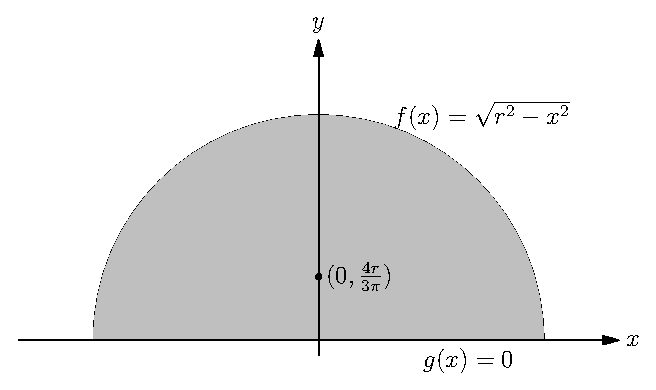
\includegraphics[width=300px]{ChapterGeom/Figures/halfdisc_cropped.eps}
\end{center}
\hfill
The mass is just half the are of a circle: $m=\frac{\pi r^2}{2}$.
Since the disc is symmetric, we already know that $\overline{x}=0$, so we only need to find $\overline{y}$. Since our $g(x)$ in this setup is the line $y=0$ and $f(x)$ is a square root, the integral simplifies nicely.

\begin{align*}
    M_x=\int_{-r}^r\frac{1}{2}\left[f(x)-g(x)\right]\left[f(x)+g(x)\right]\dif x\\
    &=\int_{-r}^r\frac{1}{2}\left(f(x)\right)^2\dif x\\
    &=\frac{1}{2}\int_{-r}^r\sqrt{r^2-x^2}\dif x\\
    &=\frac{1}{2}\left[r^2x-\frac{1}{3}x^3\right]_{-r}^r\\
    &=\frac{1}{2}\left[r^3-\frac{1}{3}r^3-\left(-r^3+\frac{1}{3}r^3\right)\right]\\
    &=\frac{2}{3}r^3
\end{align*}

Then $\overline{y}=\frac{M_x}{m}=\frac{2}{3}r^3\cdot\frac{2}{\pi r^2}=\frac{4r}{3\pi}$. Thus, the center of mass is $\left( 0, \frac{4r}{3\pi}\right)$
}{3in}
\AnswerKeyEntry{The center of mass is $\left( 0, \frac{4r}{3\pi}\right)$.}
\end{exercise}

\begin{exercise}{Center Outside \Coffeecup \Coffeecup \Coffeecup \Coffeecup}
 Can you come up with a shape whose center of mass lies outside the shape?  Find such an example, or explain why this is not possible. 
 \vspace*{3in}
 
\end{exercise}
